\documentclass{article}
\usepackage{subcaption}
\usepackage[labelformat=parens,labelsep=quad, skip=3pt]{caption}
\usepackage{graphicx}
\usepackage[font=small,labelfont=bf]{caption}
\usepackage{geometry}

\geometry{
 a4paper,
 left=0mm,
 top=0mm,
 }

\begin{document}



\begin{figure}[htp]
 \centering
\begin{subfigure}{.33\textwidth}
 \caption{DIC - GLODAPv2}
 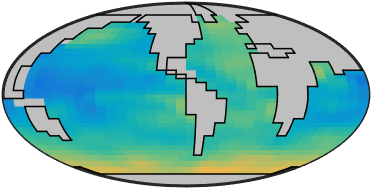
\includegraphics[width=0.95\linewidth]{../separate_figures/OBSERVATIONS/surface_TCO2.png}
 \label{fig:nutrients1}
\end{subfigure}%
\begin{subfigure}{.33\textwidth}	
 \caption{DIC -  - cGEnIE}
 \includegraphics[width=0.95\linewidth]{../separate_figures/BIOGEM/ocn_DIC.png}
 \label{fig:carbon1}
\end{subfigure}%
\begin{subfigure}{.33\textwidth}
 \caption{DIC - EcoGEnIE}
 \includegraphics[width=0.95\linewidth]{../separate_figures/ECOGEM/ocn_DIC.png}
 \label{fig:carbon2}
\end{subfigure}
\\[+0.2cm]
\begin{subfigure}{.5\textwidth}
 
\includegraphics[width=0.95\linewidth]{../separate_figures/ECOGEM/ocn_DIC_clrbr.png}
\end{subfigure}
\begin{subfigure}{.33\textwidth}
 \caption{Oxygen - WOA (2009)}
 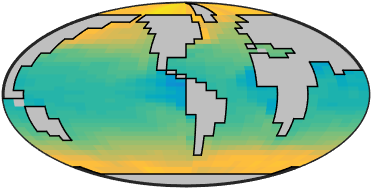
\includegraphics[width=0.95\linewidth]{../separate_figures/OBSERVATIONS/surface_o_an.png}
 \label{fig:nutrients1}
\end{subfigure}%
\begin{subfigure}{.33\textwidth}
 \caption{Oxygen - cGEnIE}
 \includegraphics[width=0.95\linewidth]{../separate_figures/BIOGEM/ocn_O2.png}
 \label{fig:carbon3}
\end{subfigure}%
\begin{subfigure}{.33\textwidth}
 \caption{Oxygen - EcoGEnIE}
 \includegraphics[width=0.95\linewidth]{../separate_figures/ECOGEM/ocn_O2.png}
 \label{fig:carbon4}
\end{subfigure}
\\[+0.2cm]
\begin{subfigure}{.5\textwidth}
 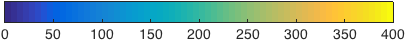
\includegraphics[width=0.95\linewidth]{../separate_figures/ECOGEM/ocn_O2_clrbr.png}
\end{subfigure}
\begin{subfigure}{.33\textwidth}
 \caption{Alkalinity - GLODAPv2}
 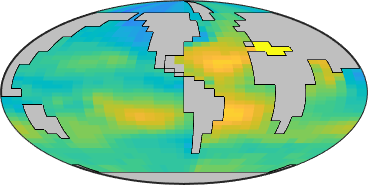
\includegraphics[width=0.95\linewidth]{../separate_figures/OBSERVATIONS/surface_TALK.png}
 \label{fig:nutrients1}
\end{subfigure}%
\begin{subfigure}{.33\textwidth}
 \caption{Alkalinity - cGEnIE}
 \includegraphics[width=0.95\linewidth]{../separate_figures/BIOGEM/ocn_ALK.png}
 \label{fig:carbon3}
\end{subfigure}%
\begin{subfigure}{.33\textwidth}
 \caption{Alkalinity - EcoGEnIE}
 \includegraphics[width=0.95\linewidth]{../separate_figures/ECOGEM/ocn_ALK.png}
 \label{fig:carbon4}
\end{subfigure}
\\[+0.2cm]
\begin{subfigure}{.5\textwidth}
 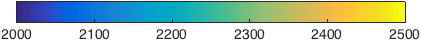
\includegraphics[width=0.95\linewidth]{../separate_figures/ECOGEM/ocn_ALK_clrbr.png}
\end{subfigure}
\end{figure}

\end{document}